%%==================================================================%%
%% Author : Tejedo Gonz�lez, Daniel                                 %%
%%          S�nchez Barreiro, Pablo                                 %%
%% Version: 1.0, 27/11/2012                                         %%                   %%                                                                  %%
%% Memoria del Proyecto Fin de Carrera                              %%
%% Gram�tica,  archivo raiz                                       %%
%%==================================================================%%

\chapterheader{Creaci�n de la gram�tica}{Creaci�n de la gram�tica}
\label{chap:gramatica}

Una vez definida la sintaxis abstracta de nuestro lenguaje, el siguiente paso era definir la sintaxis concreta de nuestro lenguaje, que en nuestro caso ser�a una sintaxis textual. Para ello hicimos uso de la herramienta EMFText. Este cap�tulo describe el proceso de desarrollo de dicha sintaxis textual concreta de acuerdo al proceso impuesto por EMFText.

\chaptertoc

%%=================================================================%%
%% NOTA(Pablo) : Lo mismo que con el cap�tulo 3, escribe una       %% 
%%               peque�a introducci�n al cap�tulo                  %%
%%=================================================================%%

\section{Introducci�n}
\label{sec:gram:introduccion}
%%==================================================================%%
%% Author : Tejedo González, Daniel                                 %%
%%          Sánchez Barreiro, Pablo                                 %%
%% Version: 1.0, 27/11/2012                                         %%
%% Version: 2.0, 09/03/2013                                         %%
%%                                                                  %%
%% Memoria del Proyecto Fin de Carrera                              %%
%% Gramática, Introduccion                                          %%
%%==================================================================%%


De acuerdo con la metodolog��a impuesta por la Ingenier�a de Lenguajes Dirigida por Modelos, el siguiente paso para desarrollar el lenguaje HCL pasa por desarrollar una sintaxis textual que sea capaz de vincular el metamodelo construido con las l�neas de c�digo que escribamos en nuestro lenguaje.  Esta sintaxis textual se construye a trav�s de una gram�tica, en la que especificamos una serie de reglas para cada una de las metaclases, de modo que esas reglas satisfagan la sintaxis y los requisitos de nuestro lenguaje. 

%%==================================================================%%
%% NOTA(Pablo): Cuando llegues a la parte en la cual hablas de      %%
%%              requisitos insertas esto                            %%
%%==================================================================%%

Los requisitos que nuestra gram�tica debe cumplir ya estaban pr�cticamente definidos, pues la gram�tica BNF definida por el profesor Pablo S�nchez, mostrada en la Figura~\ref{fig:constraintBNF}, es m�s o menos la misma que hemos tenido que implementar (con la salvedad que a�ade cambiar de lenguaje BNF a EMFText).

No obstante, hubo que a�adir una serie de consideraciones adicionales para refinar dicha gram�tica. Concretamente, tuvimos que a�adir los siguientes requisitos a la notaci�n BNF de nuestra gram�tica:

\begin{itemize}
    \item Deb�a permitirse la posibilidad de especificar prioridad en las operaciones, es decir, de poder delimitar las operaciones con par�ntesis que denoten el orden de realizaci�n de las mismas.
    \item Todo fichero de especificaci�n de restricciones debe comenzar con una l�nea que indique la ruta donde se encuentra el �rbol de caracter�sticas al que han de aplicarse las restricciones. La sintaxis de este aspecto ser� $import ruta$, donde ruta es una direcci�n que indique un fichero en nuestro computador.
    \item Todas las restricciones han de separarse entre ellas mediante el car�cter `\texttt{;}'.
\end{itemize}

%%==================================================================%%
%% NOTA(Pablo): y luego sigue con la introducción                   %%
%%==================================================================%%

Para hablar de la gram�tica, el cap�tulo se estructurar� del siguiente modo: Tras esta introducci�n, habr� una secci�n en la que se hablar� de la implementaci�n de la gram�tica. Se explicar� paso a paso cada una de las l�neas que la componen, adem�s de su relaci�n con el metamodelo. A continuaci�n, se hablar� en otra secci�n de las pruebas a las que fue sometida la gram�tica para corroborar su correcto funcionamiento.

%%=================================================================%%
%% NOTA(Pablo): Los requisitos de la gram�tica quedan 
%%              pr�cticamente definidos en el art�culo que te 
%%              mand�, y que est� descrita en el cap�tulo 
%%              anterior, por tanto no hace falta enrrollarse. 
%%              Se puede fusionar con la secci�n de introducci�n
%%=================================================================%%
%%
%% \section{Captura de requisitos}
%% \label{sec:gram:requisitos}
%% %%==================================================================%%
%% Author : Tejedo Gonz�lez, Daniel                                 %%
%%          S�nchez Barreiro, Pablo                                 %%
%% Version: 1.0, 25/11/2012                                         %%
%% Version: 2.0, 06/02/2013                                         %%
%%                                                                  %%
%% Memoria del Proyecto Fin de Carrera                              %%
%% Sintaxis abstracta, requisitos                                   %%
%%==================================================================%%

El primer paso para desarrollar nuestro lenguaje era conocer qu� aspecto deb�a tener nuestro lenguaje y qu� restricciones deb�a satisfacer. Es decir, en primer lugar debemos realizar un proceso que podemos denominar de captura de requisitos para poder comprender qu� es lo que tiene que hacer exactamente el lenguaje que se pretende crear.

Concretamente nuestro lenguaje hab�a sido pr�cticamente definido por el profesor Pablo S�nchez, del Departamento de Matem�ticas, Estad�stica y Computaci�n de la Universidad de Cantabria, mediante notaci�n BNF. Las ideas subyacentes a dicho lenguaje son las que se describen a continuaci�n.

%%==================================================================%%
%% NOTA(Pablo): Aqu� traduce la secci�n III del art�culo que te
%%              env�o adjunto. Si te hacen falta las fuentes del
%%              art�culo, me las pides.
%%
%%              Traduce primero del ingl�s y luego lo repasas y lo
%%              reescribes para que suene a castellano
%% 
%%              Si en la secci�n III no aparecen las razones por 
%%              las cuales una caracter�stica es clonable, buscar 
%%              en qu� parte del art�culo aparecen y explicarlo

%%==================================================================%%

Adem�s nuestro lenguaje deb�a permitir vincular un un modelo de caracter�sticas sobre el cual se definir�n un conjunto de restricciones externas. Este modelo se utilizar�, por ejemplo, para comprobar que los s�mbolos que aparecen como nombres de caracter�sticas en las restricciones se refieren a caracter�sticas que realmente existen en el �rbol de caracter�sticas. Por ejemplo, una restricci�n del tipo $AdvancedHeating => Heating$ carecer�a de sentido si algunas de las caracter�sticas $AdvancedHeating$ o $Heating$ no apareciesen en el �rbol de caracter�sticas sobre el cual estamos definiendo restricciones.

%%======================================================================================%%
%% NOTA(Pablo): Esto posiblemente sobre al introducir la traducci�n de la Secci�n III.
%%              Si es as�, eliminarla.
%%              Si los conceptos de restricci�n con contexto y operaci�n cuantificada
%%              no apareciesen, meter esta clasificaci�n pero resumida
%%======================================================================================%%
%%
%% De entre todos esos requisitos b�sicos, es necesario entrar en detalle en el n�mero 3
%% y enumerar la lista de operaciones que pueden ser definidas por nuestro lenguaje. Se
%% pueden clasificar en los siguientes tipos: \\
%%
%% - L�gicas: Son operaciones cuyos operandos han de ser caracter�sticas sin
%%   cardinalidad (tambi�n llamadas caracter�sticas simples), y que se evaluan a
%%   verdadero o falso. Entre las operaciones l�gicas encontramos las cl�sicas not,
%%   and, or, xor e implica.
%%
%% - Num�ricas: Sus operandos han de ser caracter�sticas con cardinalidad (tambi�n
%%   llamadas caracter�sticas m�ltiples) o simplemente n�meros. Su resultado se evalua
%%   con un valor num�rico. Las operaciones num�ricas a implementar son la suma, resta,
%%   multiplicaci�n y divisi�n.
%%
%% - Comparativas: Sus operandos han de ser caracter�sticas m�ltiples o simplemente n�meros,
%%   pero su resultado se evalua con un valor booleano. Las operaciones de comparaci�n a
%%   implementar son igual que, mayor que, menor que, distinto que, mayor o igual que y menor
%%   o igual que.
%%
%% - Operaci�n de contexto: Operaci�n que permite hacer referencia a una caracter�stica
%%   hija de otra caracter�stica. Esta operaci�n tiene sentido para seleccionar
%%   caracter�sticas cuyo nombre pueda estar repetido pero que tengan contextos diferentes.
%%   Por ejemplo, en el modelo de caracter�sticas SmartHome de la figura \ref{figsmarthome}
%%   podemos observar que la caracter�stica HeaterMng est� presente en muchos contextos
%%   diferentes. Esta operaci�n es necesaria para poder saber con seguridad a cual de esos
%%   contextos estamos aplicando la restricci�n.
%%
%% - Operaci�n de selecci�n: Operaci�n que corresponde a los operadores l�gicos cl�sicos
%%   "para todo" o "existe", y que tiene la misma funcionalidad. Evalua si una restricci�n
%%   se cumple para todos los casos en que puede existir  o si se cumple en alguno de los
%%   casos. Por ejemplo, en el modelo de la figura \ref{figsmarthome} se podr�a evaluar una
%%   restricci�n para cada una de las habitaciones que hayan sido definidas, y saber si se
%%  cumple en todas, en alguna o en ninguna.
%%
%%======================================================================================%%

Utilizando esta informaci�n como base, procedimos a crear el correspondiente metamodelo en Ecore para nuestro lenguaje.



%%
%%=================================================================%%

\section{Implementaci�n de la Gram�tica}
\label{sec:gram:design}
%%==================================================================%%
%% Author : Tejedo Gonz�lez, Daniel                                 %%
%%          S�nchez Barreiro, Pablo                                 %%
%% Version: 1.0, 27/11/2012                                         %%                   %%                                                                  %%
%% Memoria del Proyecto Fin de Carrera                              %%
%% Gram�tica,  dise�o                                       %%
%%==================================================================%%

Una vez han sido definidas las caracter�sticas que queremos que nuestra sintaxis textual posea, el siguiente paso es dise�ar una gram�tica que se ajuste a ellas. 

La parte m�s trivial e inmediata del dise�o de la gram�tica es la concerniente a la implementaci�n de las operaciones, pues las producciones necesarias simplemente requieren la inclusi�n de los operandos involucrados y los caracteres que deseemos que definan la operaci�n. La figura \ref{figopers} muestra la implementaci�n de estas operaciones. 

\begin{figure}[t]
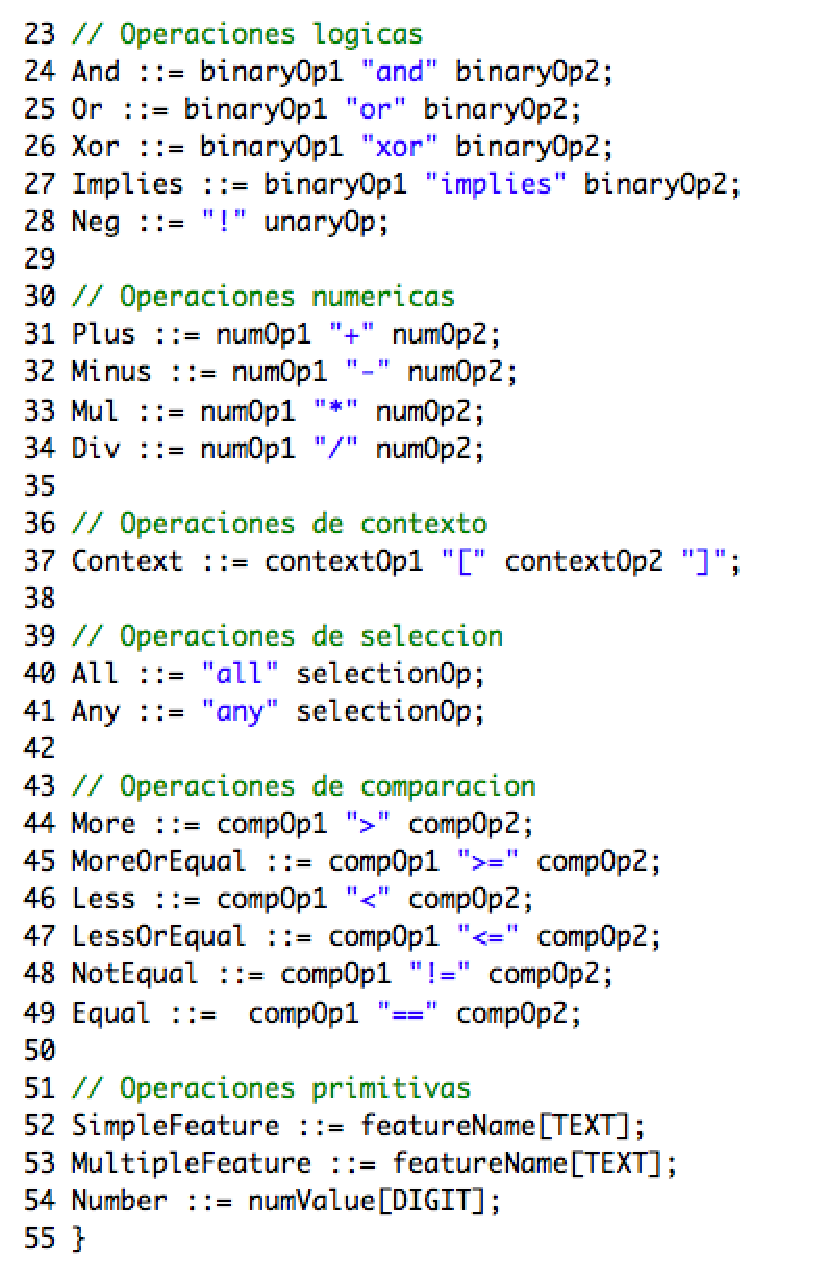
\includegraphics[scale=0.7]{gramatica/operaciones.eps}
\caption{Implementaci�n de las operaciones de nuestro editor com EMFText}
\label{figopers}
\end{figure}

S� que cabe comentar con respecto a las operaciones las �ltimas l�neas, que muestran la asignaci�n de valor a las hojas de nuestros �rboles parseados. En esas l�neas estamos indicando que los atributos de las instancias de clase Number van a ser n�meros, y que los atributos de las instancias de las clases SimpleFeature y MultipleFeature van a ser palabras.

La parte m�s complicada corresponde a la implementaci�n del inicio de la gram�tica y de las producciones que conducen a la misma. Pero antes de mostrar la figura con esta parte de la gram�tica conviene explicar el problema que llev� a realizar los cambios en el metamodelo mencionados en el cap�tulo anterior. Este problema surgi� a la hora de implementar las operaciones con prioridad, es decir, la inclusi�n de los par�ntesis.

El inconveniente es que el tipo de gram�tica LL que implementa EMFText hac�a imposible tomar una decisi�n sobre hacia qu� elemento seguir parseando en caso de encontrarnos con un par�ntesis. La mejor soluci�n que se nos ocurri� para evitar este problema fue la adici�n de diversas clases y relaciones auxiliares en el metamodelo, cuya �nica funci�n es estructural y de apoyo a la gram�tica. Gracias a ellas y a una mejor definici�n de las producciones conseguimos evitar esos problemas de parsing y podemos llevar a cabo las operaciones de prioridad con par�ntesis.

Las clases a�adidas para solventar esta situaci�n fueron las siguientes: BoolPriorityOperand1, BoolPriorityOperand2, NumPriorityOperand1, NumPriorityOperand2, BoolOperandChoices y NumOperandChoices. Las relaciones a�adidas fueron boolPriorityOp1, boolPriorityOp2, numPriorityOp1 y numPriorityOp2.

Una situaci�n similar fue la que propici� que las operaciones Context, All y Any hayan sido dise�adas tal y como presenta el metamodelo, ya que que la particular sintaxis de estas (diferente a las dem�s que siguen el mismo esquema de op + char + op) tambi�n mostraba ciertos problemas de parsing. En este caso no fue necesario a�adir elementos auxiliares, sino simplemente recolocarlos para evitar estos problemas. Con esto ya se han hecho todos los cambios en el metamodelo, que alcanza en este punto su versi�n final tal como muestra la figura \ref{figmetameta}. Con respecto al metamodelo solamente quedan por comentar los m�todos que muestran algunas clases, que ser�n explicados en los pr�ximos cap�tulos ya que se usan en el proceso de validaci�n y sem�ntica.

\begin{figure}[t]
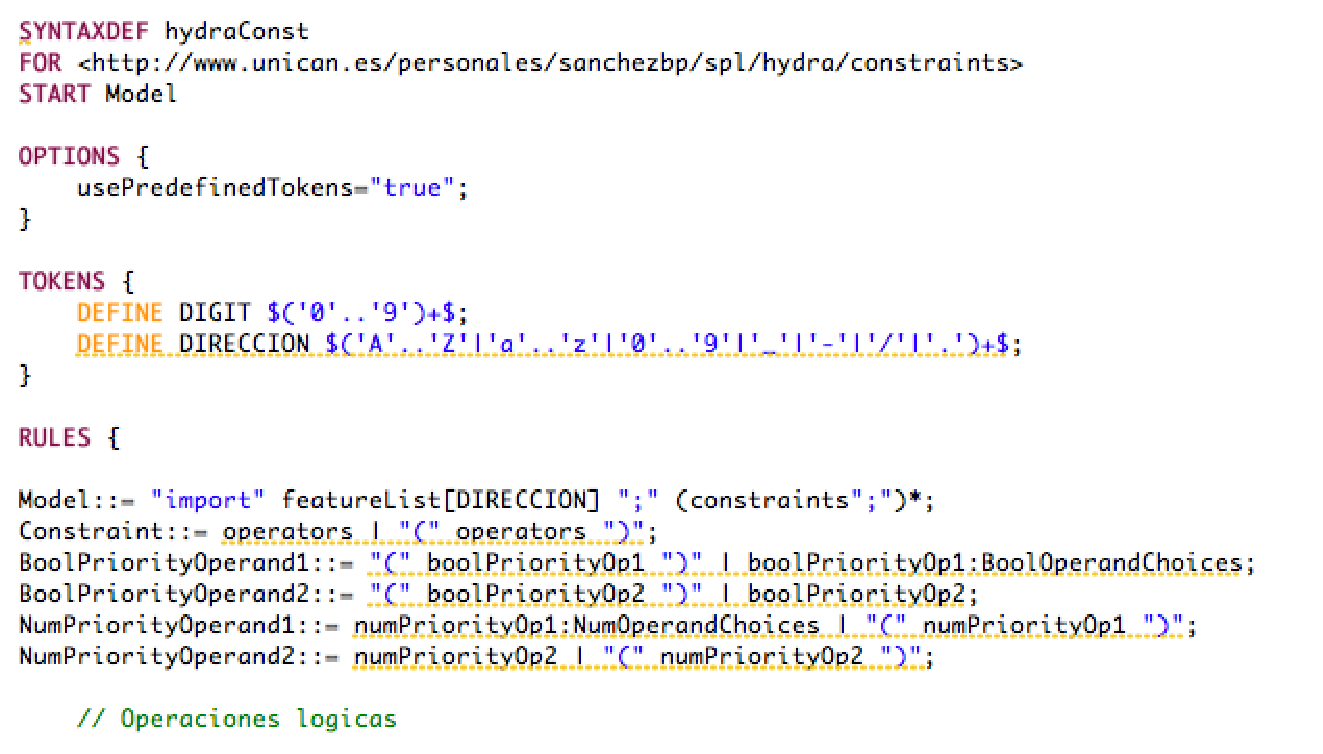
\includegraphics[scale=0.7]{gramatica/iniciogram.eps}
\caption{Implementaci�n del inicio de la gram�tica con EMFText. Con la figura \ref{figopers} se completa la gram�tica}
\label{figinitgram}
\end{figure}

Una vez comentados estos detalles es momento de explicar el inicio de la gram�tica, que se muestra en la figura \ref{figinitgram}. 

En la primera l�nea y mediante la cla�sula SYNTAXDEF indicamos la extensi�n que queremos que tengan los ficheros escritos en nuestro lenguaje. En nuestro caso nos hemos decantado por la terminaci�n .hydraConst. En la segunda l�nea y mediante la cla�sula FOR se indica la URI del metamodelo. Una URI es un formato de direcci�n interno de Eclipse, que se usa para localizar otros ficheros en el workspace. En la tercera l�nea, delimitada por la cla�sula START, indicamos a la gram�tica que la clase inicial de nuestro metamodelo (y la que ser� la raiz en todos los �rboles parseados) es Model.

El bloque OPTIONS permite activar algunas opciones de configuraci�n que incluye EMFText. En nuestro caso la �nica que tiene utilidad es usePredifinedTokens, que permite ahorrarnos la definici�n del token text. El bloque TOKENS sirve para definir los tokens de nuestra gram�tica. En nuestro caso usaremos 3: DIGIT para asignar al valor num�rico, TEXT para asignar a las caracter�sticas y DIRECCION para asignar la direcci�n f�sica del modelo de caracter�sticas.

Por �ltimo, el bloque RULES permite crear las producciones. Como inicial, tal y como se especific� en los requisitos, exigimos un import y una direcci�n, que ser� almacenada en el atributo featureList de la clase Model. En la l�nea inicial tambi�n se indica, mediante una expresi�n regular, que el n�mero de restricciones a definir puede ser tan grande como se desee y que estas deben acabar con el car�cter '';'' .

La l�nea de producci�n de Constraint diferencia entre operaciones con prioridad y sin ella. Sin el problema comentado de EMFText la gram�tica podr�a quedar as�, pero para solucionarlo nos vemos obligado a incluir las cuatro l�neas siguientes, cuya �nica funci�n es solventar esa situaci�n. El resto de la gram�tica continuar�a en la figura \ref{figopers} mostrada anteriormente, y ah� terminar�a.






\section{Pruebas}
\label{sec:gram:pruebas}
%%==================================================================%%
%% Author : Tejedo Gonz�lez, Daniel                                 %%
%%          S�nchez Barreiro, Pablo                                 %%
%% Version: 1.0, 27/11/2012                                         %%                   %%                                                                  %%
%% Memoria del Proyecto Fin de Carrera                              %%
%% Gram�tica, pruebas                                       %%
%%==================================================================%%

\begin{figure}[t]
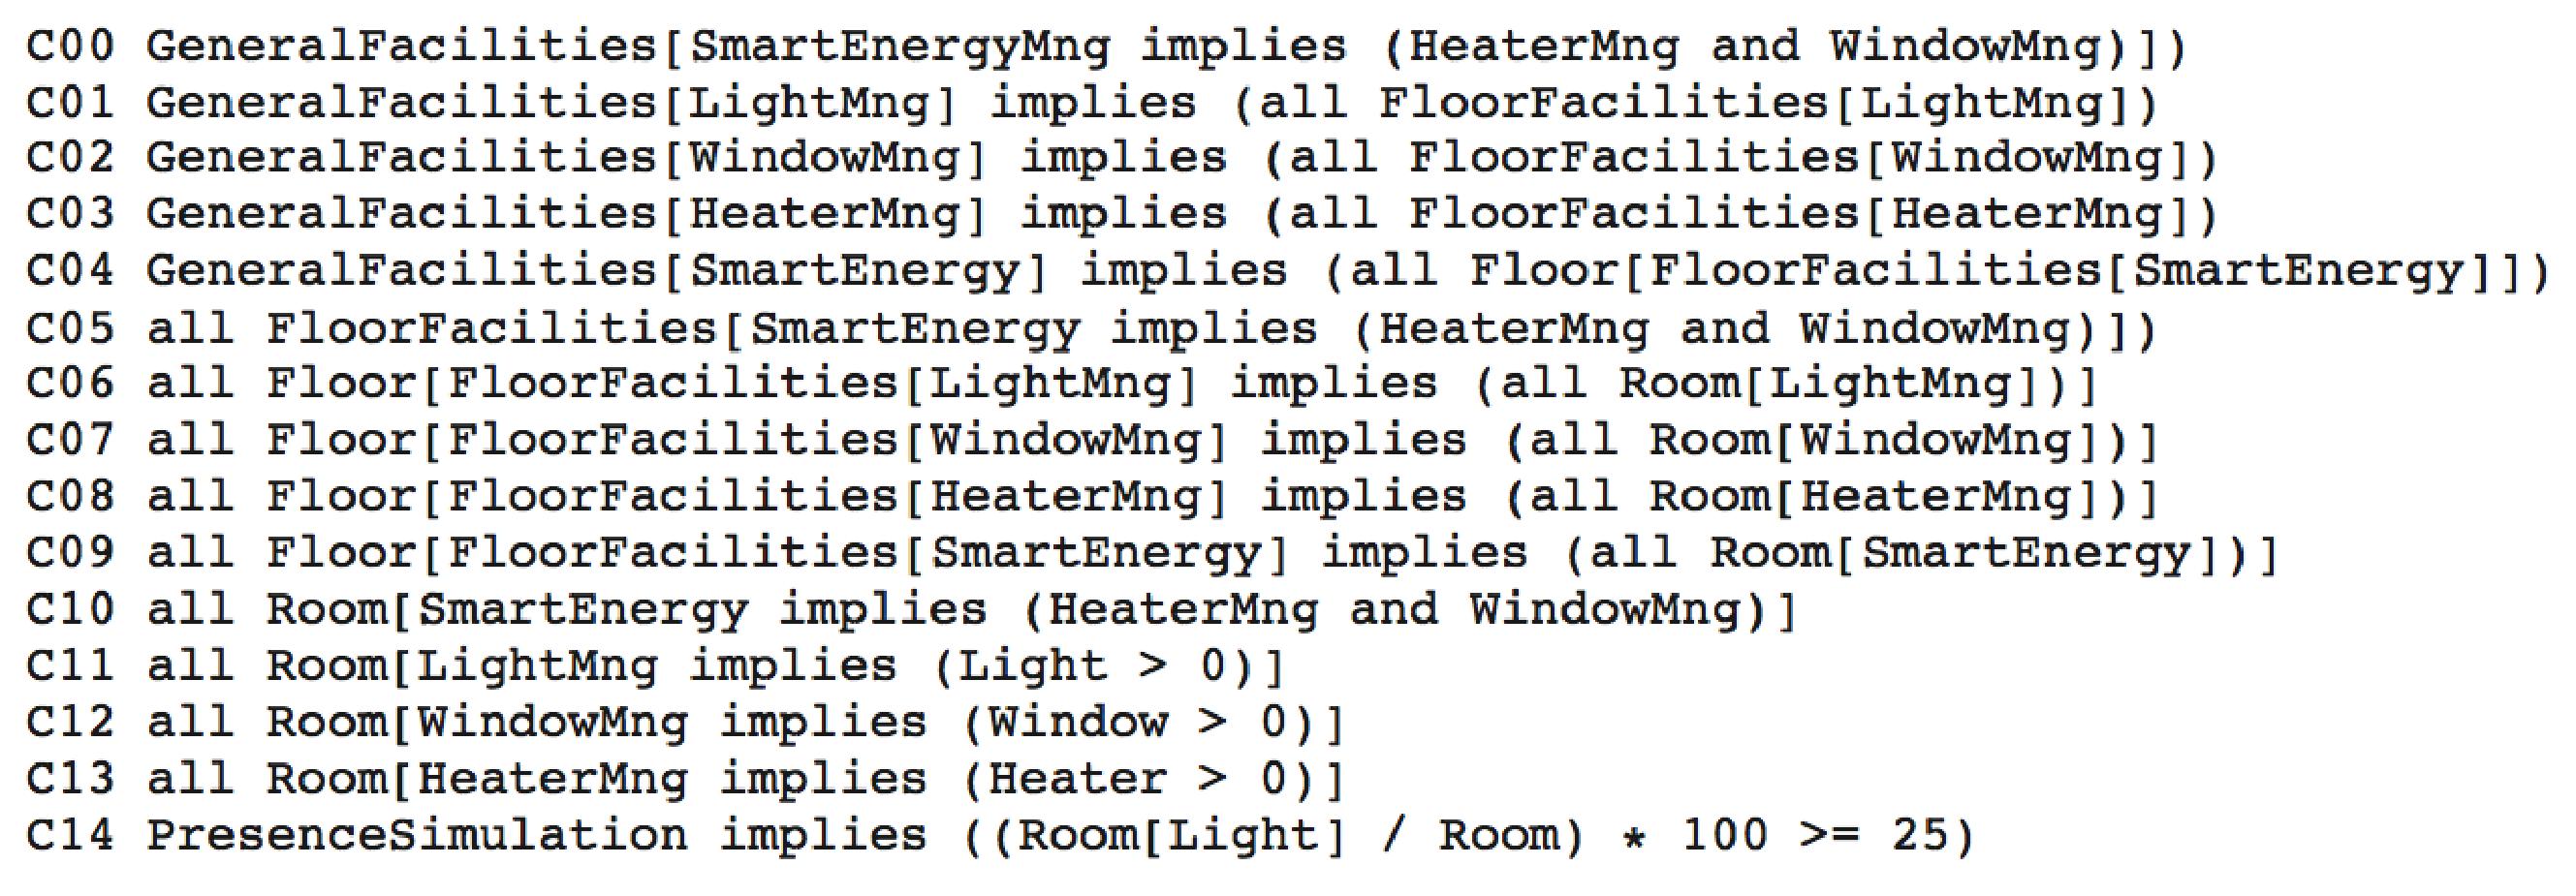
\includegraphics[scale=0.5]{gramatica/oppruebas.eps}
\caption{Bater�a de instrucciones para probar el funcionamiento de la gram�tica}
\label{figgrampruebas}
\end{figure}

Para hacer las pruebas correspondientes a la gram�tica fue de mucha utilidad la vista Outline de Eclipse, que permite obsevar el �rbol de parsing de todos los ficheros de c�digo que creemos en nuestro lenguaje. 

La bater�a de pruebas simplemente consisti� en comprobar una serie de instrucciones y observar dentro de la vista Outline si se parseaban de modo correcto. En este caso se utilizaron unas restricciones definidas en un documento previo de Hydra que conten�an todos los aspectos problem�ticos de la gram�tica, es decir, operaciones largas con prioridad y multitud de contextos. Estas instrucciones son las que se muestran en la figura \ref{figgrampruebas}. 

El resto de operaciones fueron puestas a prueba con restricciones m�s sencillitas y, como en el caso anterior, fueron exitosas. Tambi�n se usaron las instrucciones de las pruebas del cap�tulo anterior, que se pueden observar en la figura \ref{figmetains} para comprobar que el �rbol era el mismo que se cre� en ese momento.

%%=================================================================%%
%% NOTA(Pablo): A�ade una secci�n de sumario
%%=================================================================%%


\section{Sumario}
\label{sec:gram:sumario}
%%==================================================================%%
%% Author : Tejedo Gonz�lez, Daniel                                 %%
%%          S�nchez Barreiro, Pablo                                 %%
%% Version: 1.0, 25/11/2012                                         %%                   
%%                                                                  %%
%% Memoria del Proyecto Fin de Carrera                              %%
%% Sintaxis abstracta, sumario                          %%
%%==================================================================%%

Durante el presente cap�tulo se ha descrito el proceso de definici�n de la sintaxis abstracta de nuestro lenguaje. Este proceso abarca subtareas como la captura de requisitos del lenguaje, la creaci�n de un metamodelo que permita la creaci�n de sintaxis concretas apropiadas, la validaci�n de restricciones externas a ese metamodelo, y las pruebas que corroboren que todos los elementos creados funcionan correctamente. En el siguiente cap�tulo profundizaremos acerca del dise�o de la gram�tica para nuestro lenguaje, as� como de las herramientas utilizadas para implementar esa gram�tica.
